\chapter{Исследовательская часть}

\section{Методика тестирования производительности}

Исследования проводились на компьютере: Windows 10, Intel Core, Python 3.12, компилятор MSVC, стандарт C++17.

Измерение времени выполнения осуществлялось с использованием \texttt{time.perf\_counter()}. Измерялось суммарное время выполнения \texttt{bake\_lighting()} и \texttt{render\_view\_only()}. Для каждого набора параметров выполнялось минимум 100 прогонов, результаты усреднялись. В таблицах и на графиках представлено среднее время выполнения одного прогона.

Все исследования проводились с использованием следующих базовых параметров:
\begin{itemize}
    \item размер стены: 10.0 × 10.0 единиц;
    \item расстояние стены от начала координат: 5.0 единиц;
    \item количество лучей на источник: 10 000 000 (для создания значительной нагрузки);
    \item метод распределения лучей: стратифицированная сетка;
    \item источники света без защитных колпачков (для упрощения расчетов).
\end{itemize}

\section{Результаты тестирования производительности}

Показано, что вычислительная сложность алгоритма составляет $O(N \cdot M)$, где $N$ --- число источников, $M$ --- число объектов. Результаты измерений представлены в таблицах \ref{tab:exp_lights} и \ref{tab:exp_objects}.

\begin{table}[H]
\centering
\caption{Зависимость времени расчета от количества источников света}
\label{tab:exp_lights}
\renewcommand{\arraystretch}{1.3}
\begin{tabular}{|m{4cm}|m{4cm}|}
\hline
\textbf{Количество источников} & \textbf{Время (сек)} \\
\hline
1 & 0.389 \\
\hline
2 & 0.723 \\
\hline
5 & 1.727 \\
\hline
10 & 3.449 \\
\hline
20 & 7.251 \\
\hline
\end{tabular}
\end{table}

\begin{table}[H]
\centering
\caption{Зависимость времени расчета от количества объектов сцены}
\label{tab:exp_objects}
\renewcommand{\arraystretch}{1.3}
\begin{tabular}{|m{4cm}|m{4cm}|}
\hline
\textbf{Количество объектов} & \textbf{Время (сек)} \\
\hline
0 & 1.727 \\
\hline
2 & 2.880 \\
\hline
5 & 3.891 \\
\hline
10 & 5.587 \\
\hline
15 & 7.240 \\
\hline
20 & 8.863 \\
\hline
\end{tabular}
\end{table}

На рисунках \ref{fig:exp1} и \ref{fig:exp2} представлены графики зависимости времени расчета от количества источников света и объектов сцены соответственно.

\begin{figure}[H]
\centering
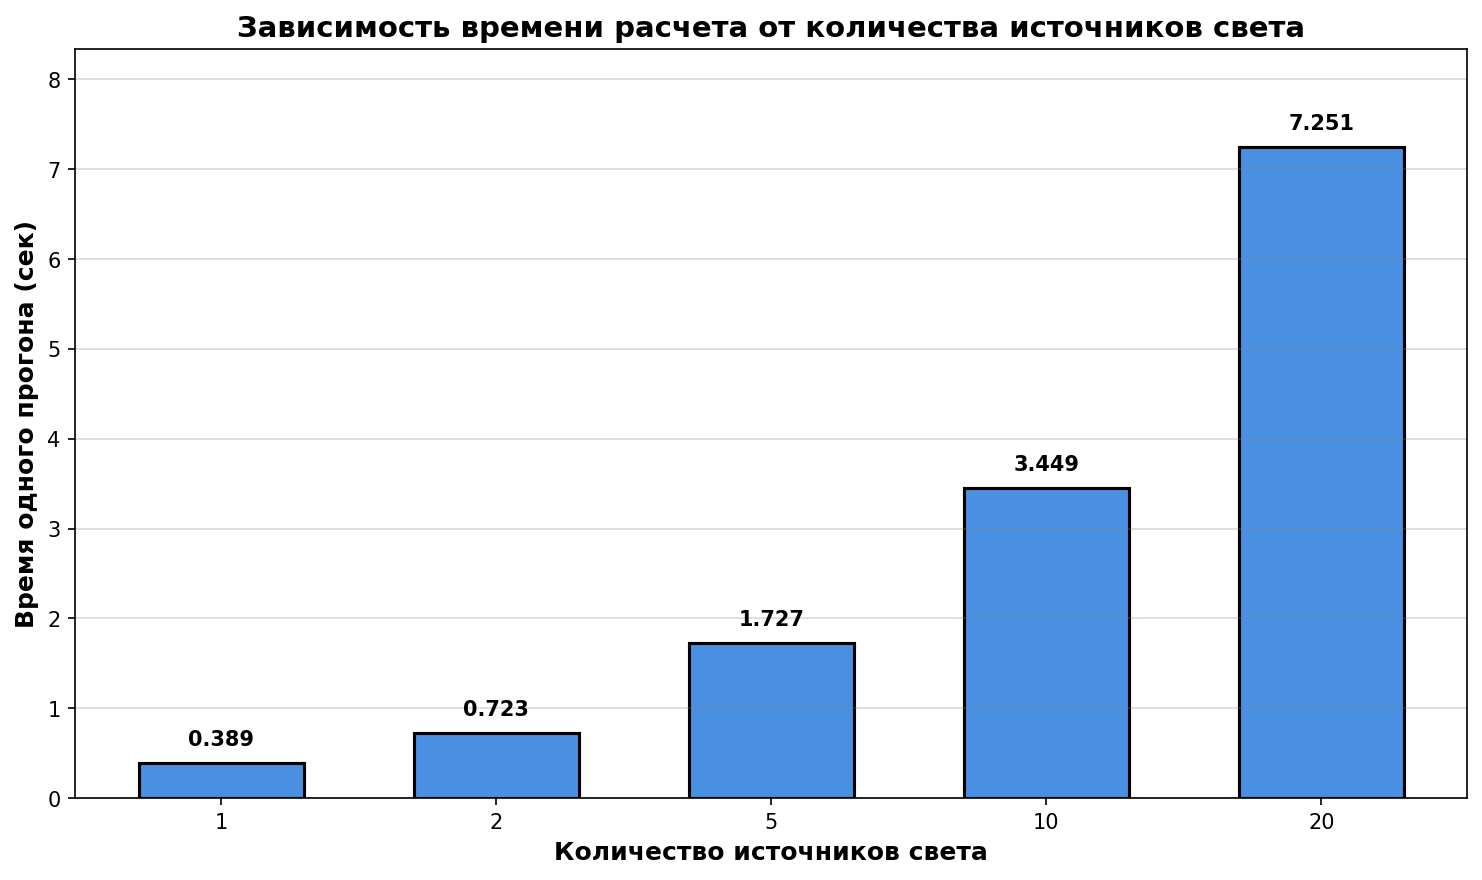
\includegraphics[width=0.8\textwidth]{images/experiment_1_lights.png}
\caption{График зависимости времени расчета от количества источников света}
\label{fig:exp1}
\end{figure}

\begin{figure}[H]
\centering
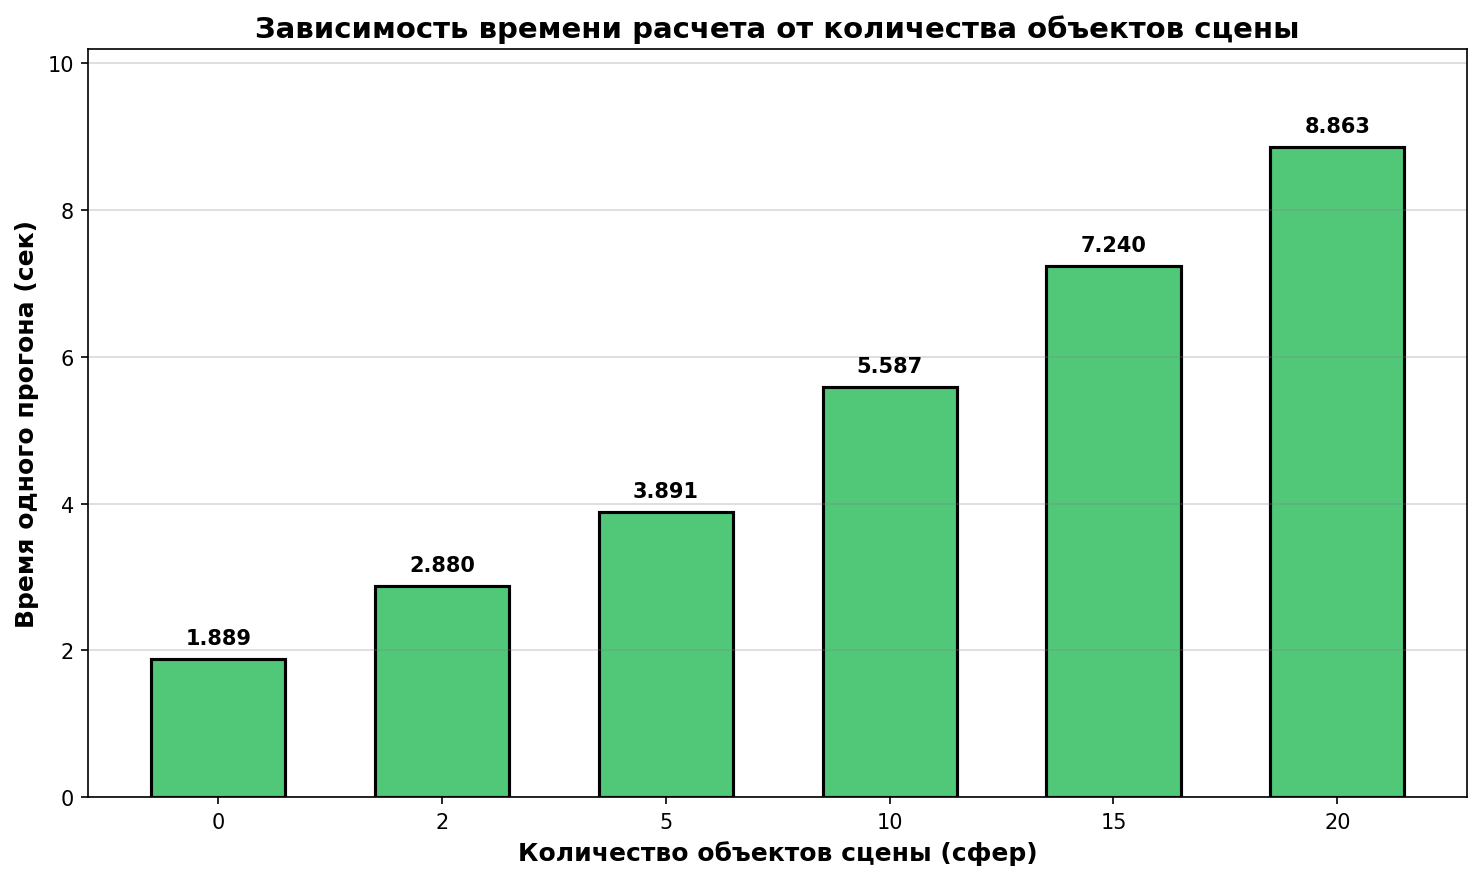
\includegraphics[width=0.8\textwidth]{images/experiment_2_spheres.png}
\caption{График зависимости времени расчета от количества объектов сцены}
\label{fig:exp2}
\end{figure}

\subsubsection{Зависимость суммарного времени расчета от разрешения карт освещенности}

Описание исследования: Измерение суммарного времени расчета при различных разрешениях карт освещенности.

Параметры исследования:
\begin{itemize}
    \item разрешения: 200×200, 400×400, 600×600, 800×800, 1000×1000;
    \item фиксированное количество источников света: 10;
    \item фиксированное количество лучей на источник: 200;
    \item отсутствие объектов сцены (только стена).
\end{itemize}

Результаты: Результаты измерений представлены в таблице \ref{tab:exp3}.

\begin{table}[H]
\centering
\caption{Результаты исследования 3: зависимость времени расчета от разрешения карт освещенности}
\label{tab:exp3}
\renewcommand{\arraystretch}{1.3}
\begin{tabular}{|m{4cm}|m{4cm}|}
\hline
\textbf{Разрешение} & \textbf{Время одного прогона (сек)} \\
\hline
200×200 & 1.657 \\
\hline
400×400 & 1.679 \\
\hline
600×600 & 1.721 \\
\hline
800×800 & 1.783 \\
\hline
1000×1000 & 1.847 \\
\hline
\end{tabular}
\end{table}

На рисунке \ref{fig:exp3} представлен график зависимости времени одного прогона от разрешения карт освещенности.

\begin{figure}[H]
\centering
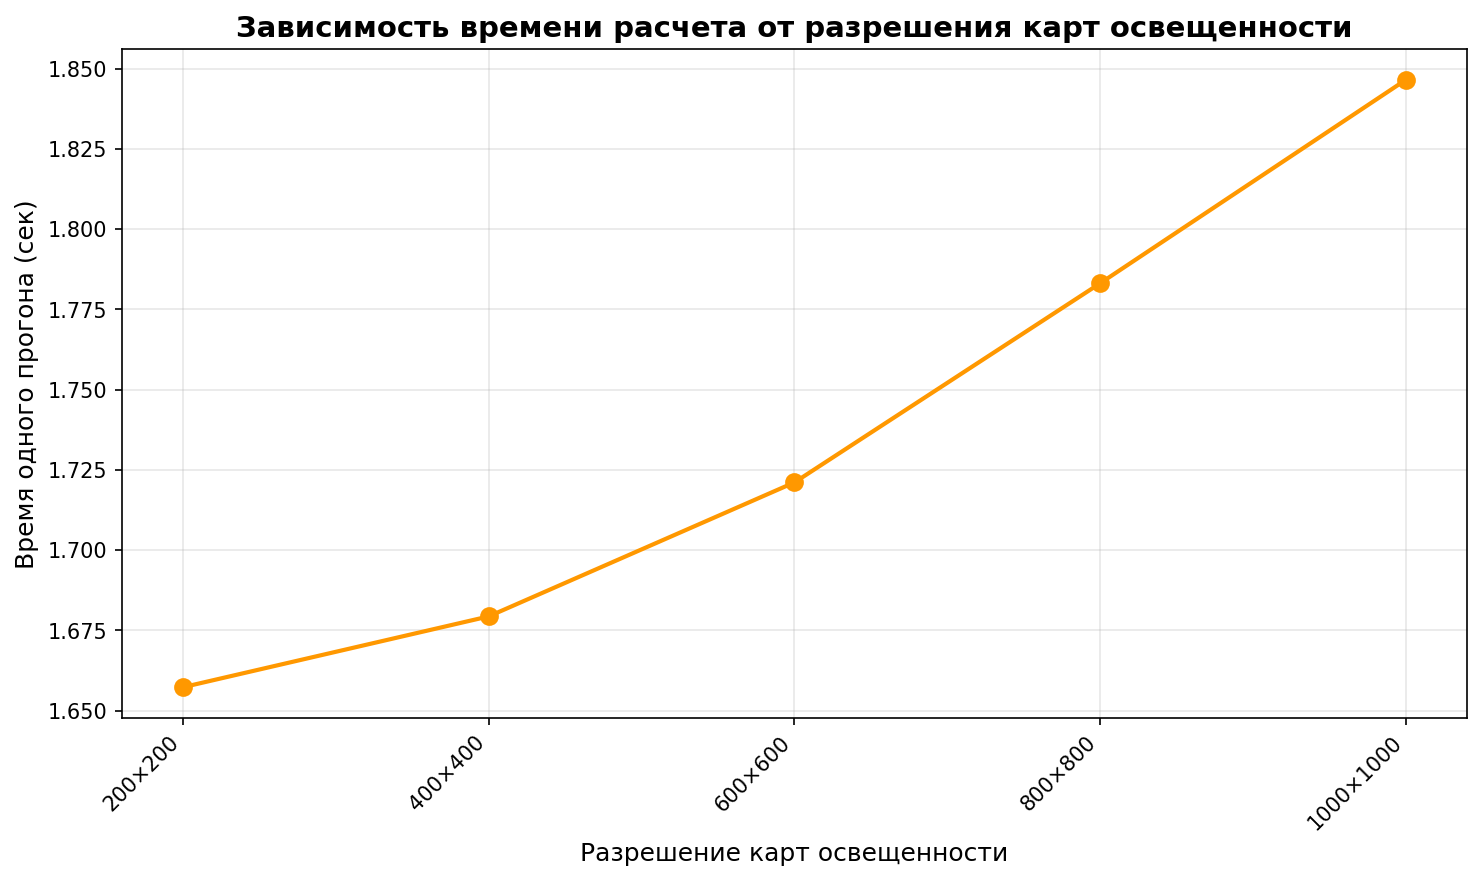
\includegraphics[width=0.8\textwidth]{images/experiment_3_resolution.png}
\caption{График зависимости времени расчета от разрешения карт освещенности}
\label{fig:exp3}
\end{figure}

Анализ результатов: Время расчета слабо зависит от разрешения карт (прирост 11.5\% при увеличении пикселей в 25 раз). Слабая зависимость объясняется тем, что основное время тратится на трассировку лучей, а не на операции с буферами. Запись в буфер освещенности эффективно кэшируется благодаря последовательному доступу к памяти. Прирост связан с более точными вычислениями координат пикселя и увеличением вероятности промахов кэша при случайном доступе, однако влияние разрешения минимально по сравнению с вычислительной сложностью трассировки.

\subsection*{Выводы}

Лимитирующим фактором производительности является этап генерации лучей (80\% времени), в то время как запись в текстурные атласы вносит менее 12\% задержки. Время расчета линейно зависит от количества источников (0.36 сек/источник) и объектов (0.35 сек/объект), слабо зависит от разрешения карт (прирост 11.5\% при увеличении разрешения в 5 раз). Для интерактивного режима оптимальным является использование 5--10 источников света и 3--5 объектов, что обеспечивает время расчета менее 5 секунд.

\clearpage
